\documentclass[aspectratio=169]{beamer}
\usefonttheme[onlymath]{serif}

\usepackage[T2A]{fontenc}
\usepackage[utf8]{inputenc}
\usepackage[english]{babel}
\usepackage{animate}
\usepackage{caption}
\usepackage{subcaption}
\usepackage{tikz}
\usepackage{cancel}
\usepackage{todonotes}


\usepackage{booktabs}
\usepackage[justification=centering]{caption}
%\setbeamercolor{block body}{gray}
%\setbeamercolor{block title}{blue}
\newcommand*{\Scale}[2][4]{\scalebox{#1}{$#2$}}%

\setbeamercolor{block title}{bg=blue!10,fg=black!50}
\setbeamercolor{block body}{bg=blue!7,fg=black}
\setbeamertemplate{bibliography item}{\insertbiblabel}
\usepackage{yfonts}
\usepackage{hyperref}
\graphicspath{{../figures/}}
\usepackage{amsmath,amsthm,amssymb}
\usepackage{bm}
\newcommand{\vect}[1]{\boldsymbol{\mathbf{#1}}}
\newcommand{\theHalgorithm}{\arabic{algorithm}}
\usepackage[ruled,vlined]{algorithm2e}

\DeclareMathOperator*{\argmin}{\arg\min\limits}

%%-----------------------------------------------------------------------
%% PRO footline
%% ----------------------------------------------------------------------
\definecolor{lightgr}{rgb}{0.7 0.7 0.7}
\definecolor{lblue}{rgb}{0.5 0.5 1}
\definecolor{progreen}{rgb}{0.329 0.659 0.404}
\definecolor{problue}{rgb}{0.294 0.447 0.686}
\makeatletter



\addtobeamertemplate{footline}{%
  \color{lblue}% to color the progressbar
  \hspace*{-\beamer@leftmargin}%
  \rule{\beamer@leftmargin}{4pt}%
  \rlap{\rule{\dimexpr
      \beamer@startpageofframe\dimexpr
      \beamer@rightmargin+\textwidth\relax/\beamer@endpageofdocument}{3pt}}
  % next 'empty' line is mandatory!

  \vspace{0\baselineskip}
  {}
}

\addtobeamertemplate{footline}{
  \leavevmode%
  \hbox{\hspace*{0.5cm}\insertsection \hspace*{0.2cm} | \hspace*{0.2cm}\insertsubsection} \hfill \hbox{\insertframenumber \hspace*{0.1cm}}
  \vskip0pt
}

\usenavigationsymbolstemplate{}

%%-----------------------------------------------------------------------
%% -----------------------------------------------------------------------

\title{Stochastic gradient algorithms from ODE
splitting perspective}

\subtitle{ICLR 2020 DeepDiffEq workshop}

\author{Daniil Merkulov, Ivan Oseledets\\
{\small \texttt{daniil.merkulov@skolkovotech.ru}, \texttt{i.oseledets@skoltech.ru}}}

\institute{Skolkovo Institute of Science and Technology} % (optional, but mostly needed)

\date{}
% \date{09 June, 2017}

% Let's get started
\begin{document}

\begingroup
\renewcommand{\insertframenumber}{}
 \begin{frame}[plain]
  \addtocounter{framenumber}{-1}
  \titlepage
 \end{frame}
\endgroup


\section{Introduction}

\begin{frame}{Finite sum problems}
\begin{equation*}\label{strang:finitesum}
    f(\vect{\vect{\theta}}) = \frac{1}{n} \sum_{i=1}^n f_i(\vect{\vect{\theta}}) \rightarrow \min_{\vect{\vect{\theta}} \in \mathbb{R}^p},
\end{equation*}

\pause

\begin{columns}

\begin{column}[t]{0.48\textwidth}
\begin{center}Discrete time\end{center}
Vanilla: $\vect{\theta}_{k+1} = \vect{\theta}_{k} - h_{k} \dfrac{1}{n} \sum\limits_{i=1}^n \nabla f_i(\vect{\vect{\theta}})$
\pause
SGD: $ \quad \vect{\theta}_{k+1} = \vect{\theta}_{k} - h_{k} \dfrac{1}{b} \sum\limits_{j=1}^b \nabla f_{i_j}(\vect{\vect{\theta}})$

\end{column}
\pause
\begin{column}[t]{0.48\textwidth}
\begin{center}Continuous time\end{center}
Vanilla: $\dfrac{d \vect{\theta}}{d t} = -\dfrac{1}{n} \sum\limits_{i=1}^n \nabla f_i(\vect{\vect{\theta}})$
\pause

SGD(?):  $\dfrac{d \vect{\theta}}{d t} = -\left(\nabla f(\vect{\vect{\theta}}) + \xi\right)$

\end{column}

\end{columns}
\pause
We propose a new view on the continuous time SGD as a first-order splitting scheme.

\end{frame}

\section{SGD as a splitting scheme}

\begin{frame}{Splitting scheme for ODE}
Simplest example of initial value problem. We have $\vect{\theta}(0) = \vect{\theta}_0$ and $\vect{\theta}(h) = ?$:

\begin{equation*}
    \frac{d \vect{\theta}}{d t} = - \frac{1}{2} \left( g_1(\vect{\theta}) + g_2(\vect{\theta})\right)
    \label{strang:gradientflow}
\end{equation*}
\pause
We split right-hand side into primitive summands and solve each problem separately with reinitialization.
$$
\frac{d \vect{\theta_1}}{d t} = - \frac{1}{2} g_1(\vect{\theta_1}), \vect{\theta_1}(0) = \vect{\theta}_0 \; \to \; \vect{\theta}_1(h);
$$
\pause
$$
\frac{d \vect{\theta_2}}{d t} = - \frac{1}{2} g_2(\vect{\theta_2}), \vect{\theta_2}(0) = \vect{\theta_1}(h) \; \to \; \vect{\theta}_2(h)
$$

\pause

First order splitting scheme: $\vect{\theta}^I(h) = \vect{\theta}_n(h)\circ \cdots \circ \vect{\theta}_1(h) \circ \vect{\theta}_0$

\end{frame}

\begin{frame}{SGD as a splitting scheme}

What if $g_1 = \nabla f_1(\vect{\theta}), g_2 = \nabla f_2(\vect{\theta})$?

\pause

\begin{table}[]
\resizebox{\textwidth}{!}{
\begin{tabular}{cccc}
\toprule
\textbf{Splitting step} & \textbf{Euler discretization} & \textbf{SGD Epoch} & \textbf{First-order splitting} \\
\midrule
$\frac{d \vect{\theta}}{d t} = -\frac{1}{2}\nabla f_1(\vect{\theta})$ & $\tilde{\vect{\theta}}_{I} = \vect{\theta}_0 - \frac{h}{2}\nabla f_1 (\vect{\theta}_0) $&$\tilde{\vect{\theta}}_{SGD} = \vect{\theta}_0 - h \nabla f_1 (\vect{\theta}_0) $&$\tilde{\vect{\theta}}_{I} = \vect{\theta}_0 - \frac{h}{2}\nabla f_1 (\vect{\theta}_0)$ \\
$\frac{d \vect{\theta}}{d t} = -\frac{1}{2}\nabla f_2(\vect{\theta}) $&$\vect{\theta}_{I} = \tilde{\vect{\theta}}_{I} - \frac{h}{2}\nabla f_2 (\tilde{\vect{\theta}}_{I}) $&$\vect{\theta}_{SGD} = \tilde{\vect{\theta}}_{SGD} - h \nabla f_2 (\tilde{\vect{\theta}}_{SGD}) $&$\vect{\theta}_{I} = \tilde{\vect{\theta}}_{I} - \frac{h}{2}\nabla f_2 (\tilde{\vect{\theta}}_{I})$ \\
\bottomrule
\end{tabular}
}
\end{table}

\pause

\begin{block}{}
Thus, we can conclude, that one epoch of SGD is just the splitting scheme for the discretized Gradient Flow ODE with $2 \cdot h$ step size ($m \cdot h$ in case of $m$ batches)
\end{block}
\end{frame}

\section{Optimization step with ODE solver}

\begin{frame}{Idea}

\begin{enumerate}
\item Consider some finite-sum problem \pause
\item Formulate corresponding ODE \pause
\item Apply first order splitting and solve local problems more precisely, than Euler (as it is done in SGD). \pause
\item Compare with SGD approximation in the same time. \pause
\end{enumerate}
\begin{table}[]
\resizebox{\textwidth}{!}{
\begin{tabular}{cccc}
\toprule
\textbf{Problem} & \textbf{Loss function} & \textbf{Batch gradient} & \textbf{Initial local ODE} \\
\midrule
Linear Least Squares & $f(\vect{\theta}) = \frac{1}{n}\sum\limits_{i=1}^m\Vert X_i \vect{\theta} - \vect{y_i} \Vert_2^2$ & $\frac{1}{b}X_i^\top( X_i \vect{\theta} - \vect{y_i})$ & $\frac{d \vect{\theta}}{d t} = - \frac{1}{n} X_i^\top( X_i \vect{\theta} - \vect{y_i})$ \\
Binary logistic regression & $\begin{aligned}f(\vect{\theta}) = -\frac{1}{n} \sum_{i=1}^n\left(y_i \ln \sigma(\vect{\theta}^\top\vect{x_i})  \right.&+ \\ \left.+ (1-y_i) \ln \left(1-\sigma(\vect{\theta}^\top\vect{x_i})\right)\right)&\end{aligned}$ & $\frac{1}{b}X_i^\top\left( \sigma\left(X_i \vect{\theta}\right) - \vect{y_i}\right)$ & $\frac{d \vect{\theta}}{d t} = - \frac{1}{n} X_i^\top\left( \sigma\left(X_i \vect{\theta}\right) - \vect{y_i}\right)$ \\
One FC Layer + softmax & $f(\Theta) = 
-\frac{1}{n} \sum\limits_{i=1}^n\log\left(\frac{\vect{y_i}^\top e^{\Theta^\top \vect{x_i}}}{\vect{1}^\top e^{\Theta^\top \vect{x_i}}}\right)$ & $ \frac{1}{b} X_i^\top\left(s(\Theta^\top X_i^\top) - Y_i \right)^\top$ & $\frac{d \Theta}{d t} = - \frac{1}{n} X_i^\top\left(s(\Theta^\top X_i^\top) - Y_i \right)^\top$\\
\bottomrule
\end{tabular}
}
\end{table}



\end{frame}

\begin{frame}{Integration of local problems}

It is important, that we can reduce dimensionality of the dynamic system via $QR$ decomposition of each batch data matrix $X_i^\top = Q_i R_i$ and substitution $\vect{\eta}_i = Q_i^\top \vect{\theta}$. 
\pause
$$
\frac{d \vect{\theta}}{d t} = - \frac{1}{n} X_i^\top( X_i \vect{\theta} - \vect{y_i}), \vect{\theta} \in \mathbb{R}^p
$$
\pause
$$
\begin{cases} \frac{d \vect{\eta_i}}{d t} = - \frac{1}{n} R_i\left(R_i^\top \vect{\eta_i} - \vect{y_i}\right), \vect{\eta_i} = Q_i^\top\vect{\theta}, \vect{\eta_i} \in \mathbb{R}^b \\ \vect{\theta}(h) = Q_i \left(\vect{\eta_i}(h) - \vect{\eta_i}(0) \right) + \vect{\theta}_0 
\end{cases}
$$
\pause
\begin{table}[]
\resizebox{\textwidth}{!}{
\begin{tabular}{llc}
\toprule
\multicolumn{1}{c}{\textbf{Initial local ODE}} & \multicolumn{1}{c}{$\mathcal{P}_i^k$} & \textbf{Integration} \\
\midrule
$\frac{d \vect{\theta}}{d t} = - \frac{1}{n} X_i^\top( X_i \vect{\theta} - \vect{y_i})$ & $\frac{d \vect{\eta_i}}{d t} = - \frac{1}{n} R_i\left(R_i^\top \vect{\eta_i} - \vect{y_i}\right), \vect{\eta_i} = Q_i^\top\vect{\theta}$ & analytical \\
$\frac{d \vect{\theta}}{d t} = - \frac{1}{n} X_i^\top\left( \sigma\left(X_i \vect{\theta}\right) - \vect{y_i}\right)$ & $\frac{d \vect{\eta_i}}{d t} = - \frac{1}{n} R_i\left(\sigma\left(R_i^\top \vect{\eta_i}\right) - \vect{y_i}\right), \vect{\eta_i} = Q_i^\top\vect{\theta}$ & \texttt{odeint} \\
$\frac{d \Theta}{d t} = - \frac{1}{n} X_i^\top\left(s(\Theta^\top X_i^\top) - Y_i \right)^\top$ & $\frac{d H_i}{dt} = - \frac{1}{n} R_i(s(H_i^\top R) - Y_i)^\top, H_i = Q_i^\top \Theta $& \texttt{odeint} \\
\bottomrule
\end{tabular}
}
\end{table}

\end{frame}

\begin{frame}{Algorithm}

\begin{algorithm}[H]
\SetAlgoLined
$\vect{\theta}_0$ - initial parameter; $b$ - batch size; $\alpha$ - learning rate; $m$- total number of batches

$h := \alpha m$

$t := 0$

\For{$k = 0,1, \ldots$}{
	\For{$i = 1,2, \ldots, m$}{
		Formulate local ODE problem $\mathcal{P}_i^k$

		$\vect{\theta}_{t+1} = $ integrate $\mathcal{P}_i^k$ given an initial value $\vect{\theta}(0) = \vect{\theta}_t$ to the step h

		$t := t+1$ 
		}
	}
\caption{Splitting optimization}
\end{algorithm}

\end{frame}

\section{Results}

\begin{frame}{Random linear system}
$10000\times500$. $b = 20$. Relative error $10^{-3}$
\begin{figure}
    \begin{subfigure}[b]{0.5\textwidth}
            \centering
            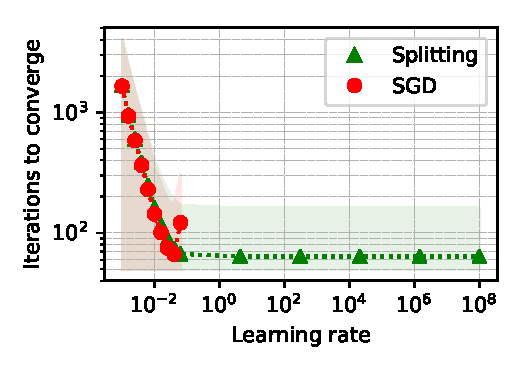
\includegraphics[width=\linewidth]{LLS_iter.pdf}
            \vspace{-25pt}
            \caption{{\small \texttt{Iterations}}}
            \vspace{-22pt}
    \end{subfigure}%
    \begin{subfigure}[b]{0.5\textwidth}
            \centering
            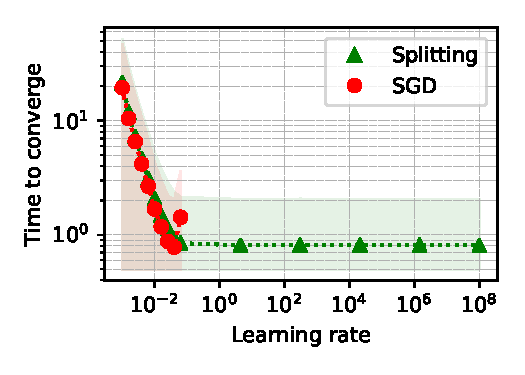
\includegraphics[width=\linewidth]{LLS_time.pdf}
            \vspace{-25pt}
            \caption{{\small \texttt{Time}}}
            \vspace{-22pt}
    \end{subfigure}%
\end{figure}
\end{frame}

\begin{frame}{Real linear system}
Tomogropy data from AIRTools II $12780\times2500$. $b = 60$. Relative error $10^{-3}$
\begin{figure}
    \begin{subfigure}[b]{0.5\textwidth}
            \centering
            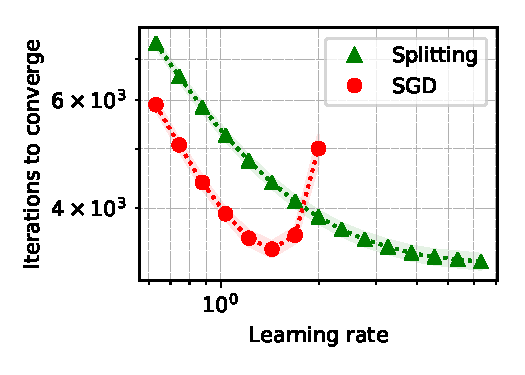
\includegraphics[width=\linewidth]{LLS_tom_iter.pdf}
            \vspace{-25pt}
            \caption{{\small \texttt{Iterations}}}
            \vspace{-22pt}
    \end{subfigure}%
    \begin{subfigure}[b]{0.5\textwidth}
            \centering
            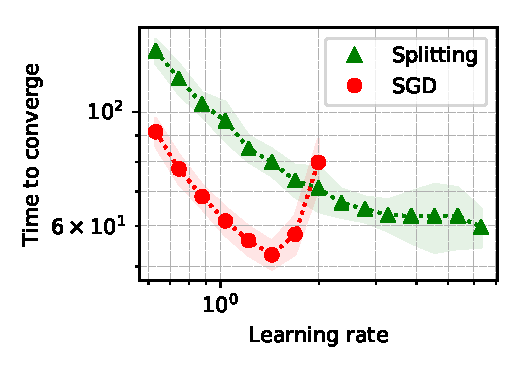
\includegraphics[width=\linewidth]{LLS_tom_time.pdf}
            \vspace{-25pt}
            \caption{{\small \texttt{Time}}}
            \vspace{-22pt}
    \end{subfigure}%
\end{figure}
\end{frame}

\begin{frame}{Binary logistic regression}
MNIST 0,1 dataset. $b = 50$. Test error $10^{-3}$
\begin{figure}
    \begin{subfigure}[b]{0.5\textwidth}
            \centering
            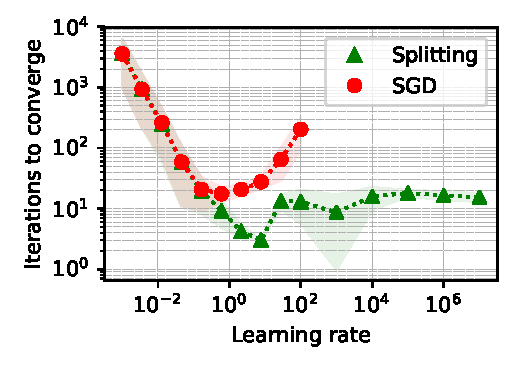
\includegraphics[width=\linewidth]{Logreg_iter.pdf}
            \vspace{-25pt}
            \caption{{\small \texttt{Iterations}}}
            \vspace{-22pt}
    \end{subfigure}%
    \begin{subfigure}[b]{0.5\textwidth}
            \centering
            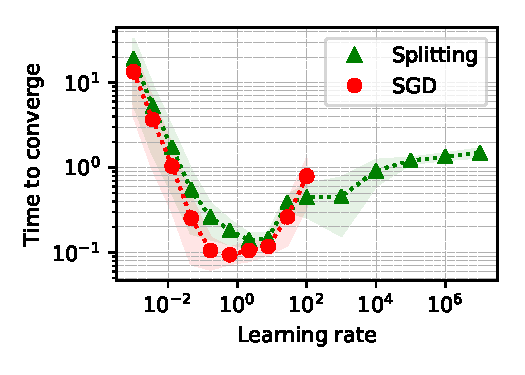
\includegraphics[width=\linewidth]{Logreg_time.pdf}
            \vspace{-25pt}
            \caption{{\small \texttt{Time}}}
            \vspace{-22pt}
    \end{subfigure}%
\end{figure}
\end{frame}

\begin{frame}{Softmax regression}
Fashion MNIST dataset. 10 classes. $28 \times 28$ images, $b = 64$. Test error $0.25$
\begin{figure}
    \begin{subfigure}[b]{0.5\textwidth}
            \centering
            \includegraphics[width=\linewidth]{{Softmax_fashion_mnist_iter_err0.25}.pdf}
            \vspace{-25pt}
            \caption{{\small \texttt{Iterations}}}
            \vspace{-22pt}
    \end{subfigure}%
    \begin{subfigure}[b]{0.5\textwidth}
            \centering
            \includegraphics[width=\linewidth]{{Softmax_fashion_mnist_time_err0.25}.pdf}
            \vspace{-25pt}
            \caption{{\small \texttt{Time}}}
            \vspace{-22pt}
    \end{subfigure}%
\end{figure}
\end{frame}




\begin{frame}{SGD vs Splitting. Iteration comparison}
\begin{figure}
    \begin{subfigure}[b]{0.35\textwidth}
            \centering
            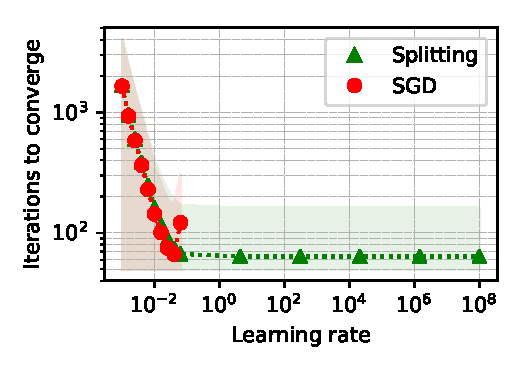
\includegraphics[width=\linewidth]{LLS_iter.pdf}
            \vspace{-25pt}
            \caption{{\small \texttt{Random LLS}}}
            \vspace{-22pt}
    \end{subfigure}%
    \begin{subfigure}[b]{0.35\textwidth}
            \centering
            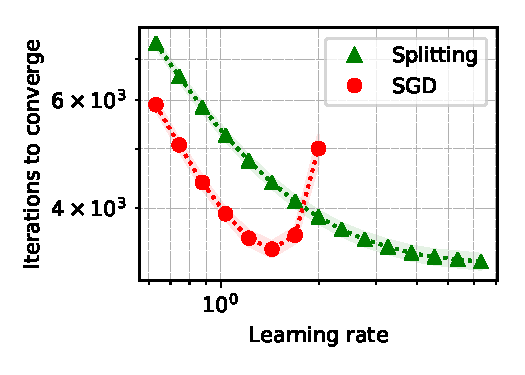
\includegraphics[width=\linewidth]{LLS_tom_iter.pdf}
            \vspace{-25pt}
            \caption{{\small \texttt{Tom LLS}}}
            \vspace{-22pt}
    \end{subfigure}%
    \vskip\baselineskip
    \begin{subfigure}[b]{0.35\textwidth}
            \centering
            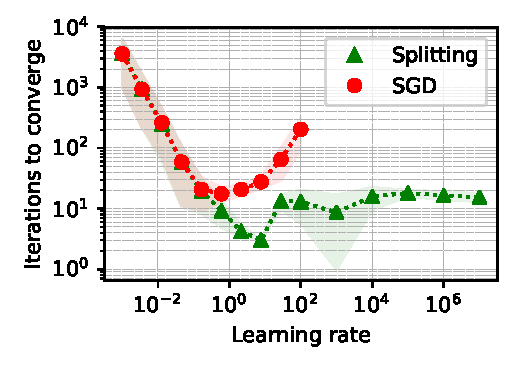
\includegraphics[width=\linewidth]{Logreg_iter.pdf}
            \vspace{-25pt}
            \caption{{\small \texttt{LogReg}}}
            \vspace{-22pt}
    \end{subfigure}%
    \begin{subfigure}[b]{0.35\textwidth}
            \centering
            \includegraphics[width=\linewidth]{{Softmax_fashion_mnist_iter_err0.25}.pdf}
            \vspace{-25pt}
            \caption{{\small \texttt{Softmax}}}
            \vspace{-22pt}
    \end{subfigure}
\end{figure}
\end{frame}

\begin{frame}{SGD vs Splitting. Time comparison}
\begin{figure}
    \begin{subfigure}[b]{0.35\textwidth}
            \centering
            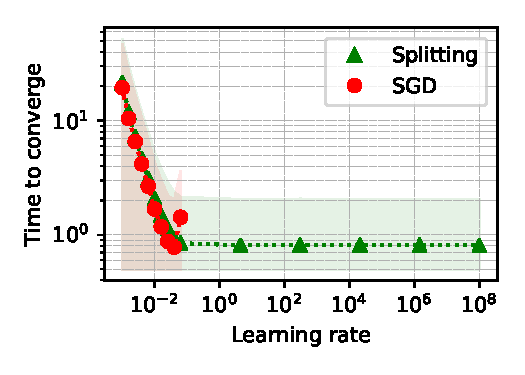
\includegraphics[width=\linewidth]{LLS_time.pdf}
            \vspace{-25pt}
            \caption{{\small \texttt{Random LLS}}}
            \vspace{-22pt}
    \end{subfigure}%
    \begin{subfigure}[b]{0.35\textwidth}
            \centering
            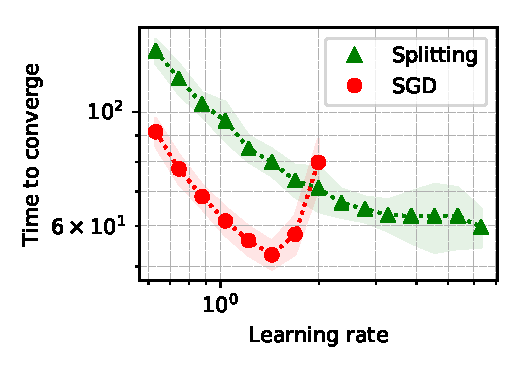
\includegraphics[width=\linewidth]{LLS_tom_time.pdf}
            \vspace{-25pt}
            \caption{{\small \texttt{Tom LLS}}}
            \vspace{-22pt}
    \end{subfigure}%
    \vskip\baselineskip
    \begin{subfigure}[b]{0.35\textwidth}
            \centering
            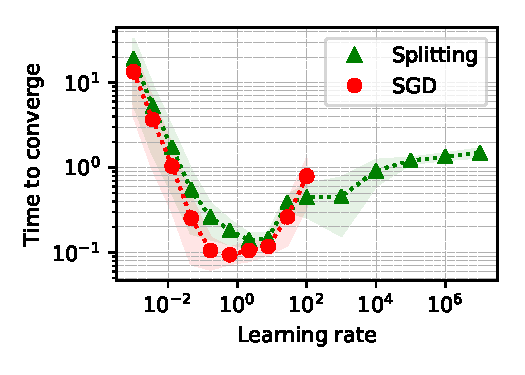
\includegraphics[width=\linewidth]{Logreg_time.pdf}
            \vspace{-25pt}
            \caption{{\small \texttt{LogReg}}}
            \vspace{-22pt}
    \end{subfigure}%
    \begin{subfigure}[b]{0.35\textwidth}
            \centering
            \includegraphics[width=\linewidth]{{Softmax_fashion_mnist_time_err0.25}.pdf}
            \vspace{-25pt}
            \caption{{\small \texttt{Softmax}}}
            \vspace{-22pt}
    \end{subfigure}
\end{figure}
\end{frame}

\begin{frame}[plain]
\begin{center}
	\Huge Thank you for your attention!

	\vfill
	Contact: \texttt{daniil.merkulov@skolkovotech.ru}
	\vfill
	Paper and code: 
	\href{https://merkulov.top/sgd_splitting}{\texttt{merkulov.top/sgd\_splitting}}

\end{center}
\end{frame}

\end{document}